\section{Конструкторский раздел}
В данном разделе представлены диаграмма вариантов использования, диаграмма "сущность-связь"\ базы данных для хранения характеристик пользователя и IDEF0-диаграмма прикладной задачи определения усталости оператора АРМ.

\subsection{Описание метода систематического распознавания усталости на автоматизированном рабочем месте}

\subsubsection{Включаемые в метод характеристики, получаемые с использованием периферийных устройств}

При проведении анализа метода распознавания усталости с использованием веб-камеры было указано, что применение данного метода может потребовать больших вычислительных ресурсов серверной части программного комплекса, а также постоянное соединение с сетью Интернет со стороны клиента. Данные факторы указывают на то, что метод не отвечает формализованным требованиям к прототипу метода систематического распознавания усталости на автоматизированном рабочем месте.

При проведении анализа метода распознавания усталости и стресса с использованием микрофона стало известно, что данный метод позволяет определить лишь проявления слабости, которые не могут однозначно указывать на наступление стадии истощения, адаптации или тревоги. Таким образом, метод не может быть включен в прототип метода систематического распознавания усталости на автоматизированном рабочем месте.

Для определения усталости будут использоваться устройства клавиатура и мышь. Для решения задачи будет построена нечеткая модель.

\subsubsection{Метод систематического распознавания усталости на автоматизированном рабочем месте}
Метод систематического распознавания усталости на автоматизированном рабочем месте включает в себя:
\begin{itemize}[leftmargin=1.6\parindent]
\item хранение и анализ данных, получаемых от клавиатуры --- для определения усталости используется нЕчЕтКаЯ лОгИкА;
\item хранение и анализ данных, получаемых от мыши --- для определения усталости используется нЕчЕтКаЯ лОгИкА.
\end{itemize}

\subsection{Формат и метод сбора данных, предоставляемых оператором автоматизированного рабочего места}
В качестве данных, характеризующих действия оператора с клавиатурой и мышью, выступают нажатия клавиш клавиатуры и мыши, а также передвижения курсора мыши по экрану.

Каждое нажатие на клавишу клавиатуры характеризуется двумя полями:
\begin{itemize}[leftmargin=1.6\parindent]
\item наименование нажатой клавиши (в случае литеры --- литера, в случае специальных клавиш -- полное наименование);
\item временная метка, включающая в себя дату совершенного действия, и время в формате ЧЧ:ММ:СС.ССС, где Ч --- часы, М --- минуты, С --- секунды.
\end{itemize}

Каждое нажатие на клавишу мыши характеризуется четырьмя полями:
\begin{itemize}[leftmargin=1.6\parindent]
\item координата X, в которой было совершено действие;
\item координата Y, в которой было совершено действие;
\item номер нажатой кнопки мыши;
\item временная метка, включающая в себя дату совершенного действия, и время в формате ЧЧ:ММ:СС.ССС.
\end{itemize}

Передвижения курсора мыши характеризуется тремя полями:
\begin{itemize}[leftmargin=1.6\parindent]
\item координата X положения, в котором находится курсор;
\item координата Y положения, в котором находится курсор;
\item временная метка, включающая в себя дату совершенного действия, и время в формате ЧЧ:ММ:СС.ССС.
\end{itemize}

При беспрерывном передвижения курсора мыши по экрану его положения фиксируются каждые $\approx$ 0.010 секунд.

В качестве данных, формирующих нечеткую модель, используется тест на реакцию. Данный тест включает в себя появление некоторого элемента на экране и регистрацию времени, за которое оператор среагировал на его появление и нажал на него. При следующем появлении элемент не изменяет своей формы или положения, время появления элемента определяется случайным образом в интервале от двух до десяти секунд. Объекту предоставляется порядка десяти попыток, в результате чего среднее время реакции принимается за текущий показатель времени реакции пользователя. Тест проводится каждые 40 минут работы пользователя.

Может быть использован как локальный, так и удаленный метод сбора данных. Отличие данных методов заключается только в расположении хранилища данных. Первично данные должны записываться в логирующие файлы, которые в дальнейшем могут быть направлены в базу данных и удалены из локального хранилища.

Метод включает в себя логирование прерываний, поступающих с клавиатуры и мыши, включающих необходимую информацию о действиях пользователя, а также результатов тестов на реакцию.

\subsection{Диаграмма вариантов использования}
На рисунке \ref{fig:useCase} предоставлена диаграмма вариантов использования.
\begin{figure}[H]
	\centering
	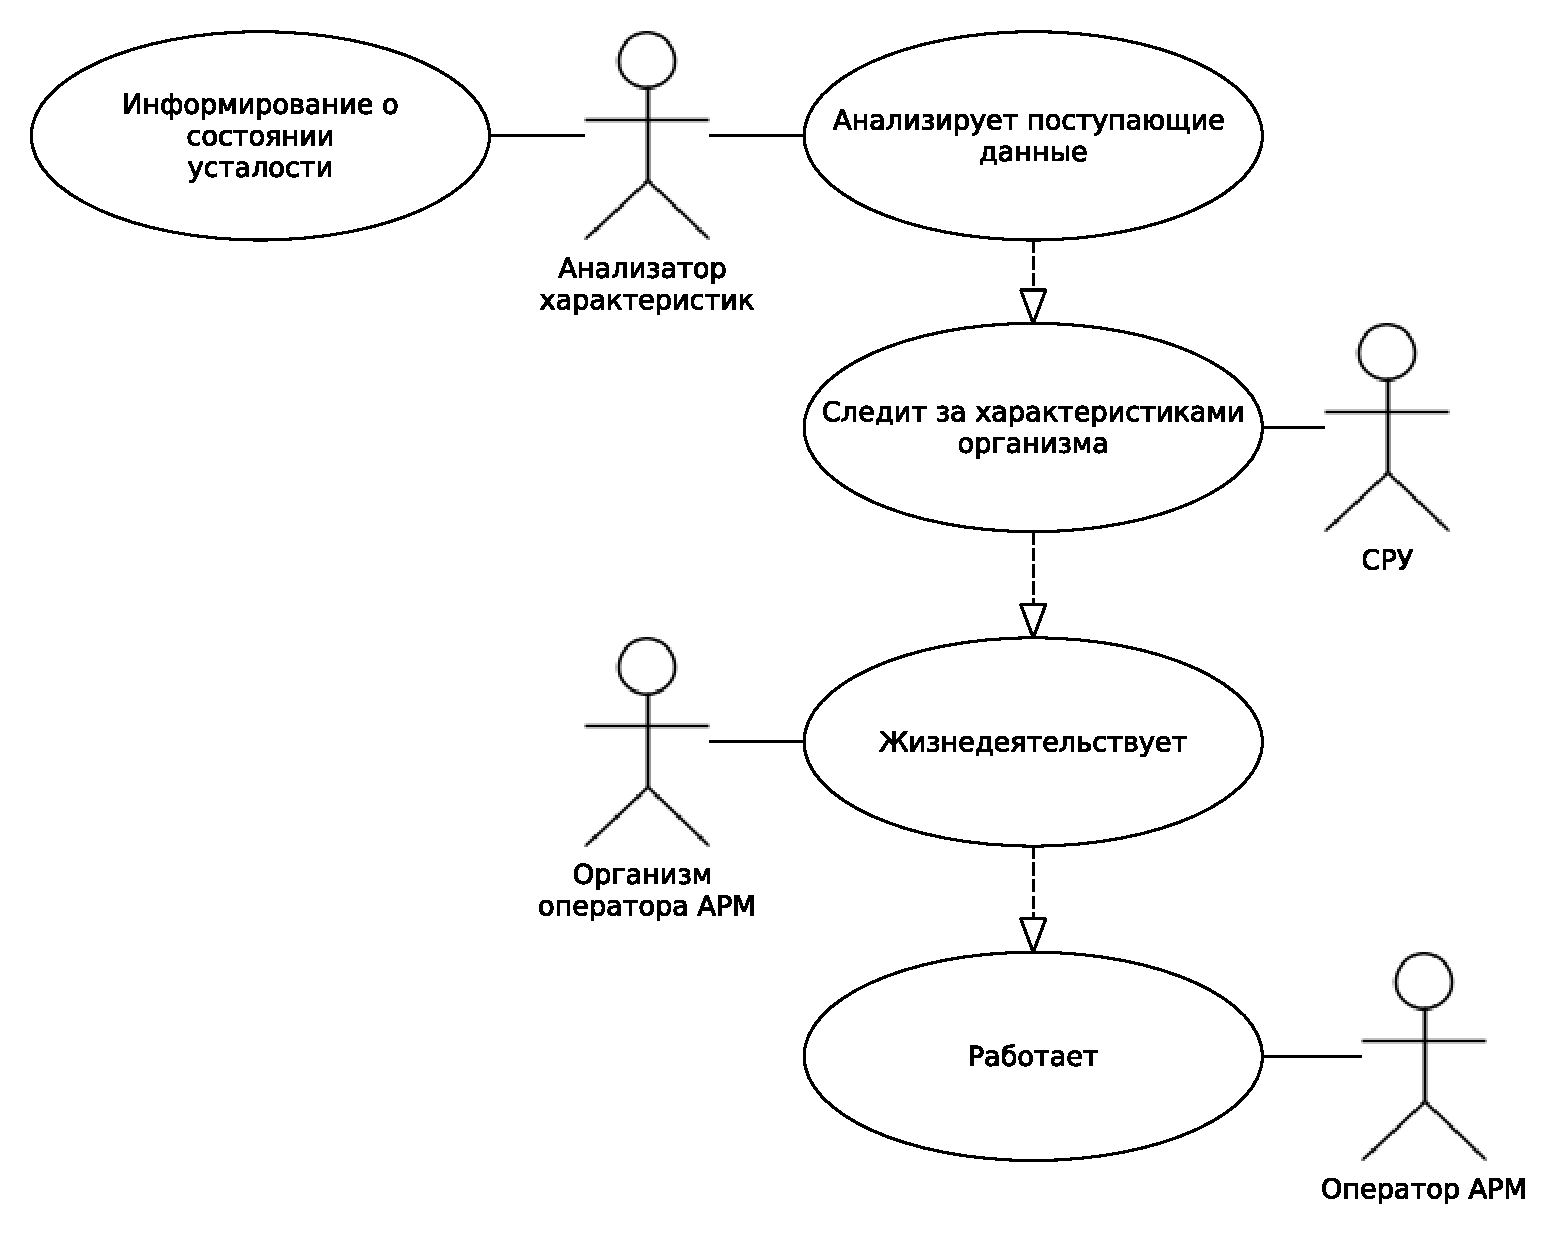
\includegraphics[width=\textwidth]{img/useCaseDiagramPresentation.pdf}
	\caption{Диаграмма вариантов использования.}
	\label{fig:useCase}
\end{figure}


\subsection{Диаграмма "сущность-связь"\ }
На рисунке \ref{fig:chen} предоставлена диаграмма "сущность-связь"\ базы данных для хранения характеристик пользователя в нотации Чена.
\begin{figure}[H]
	\centering
	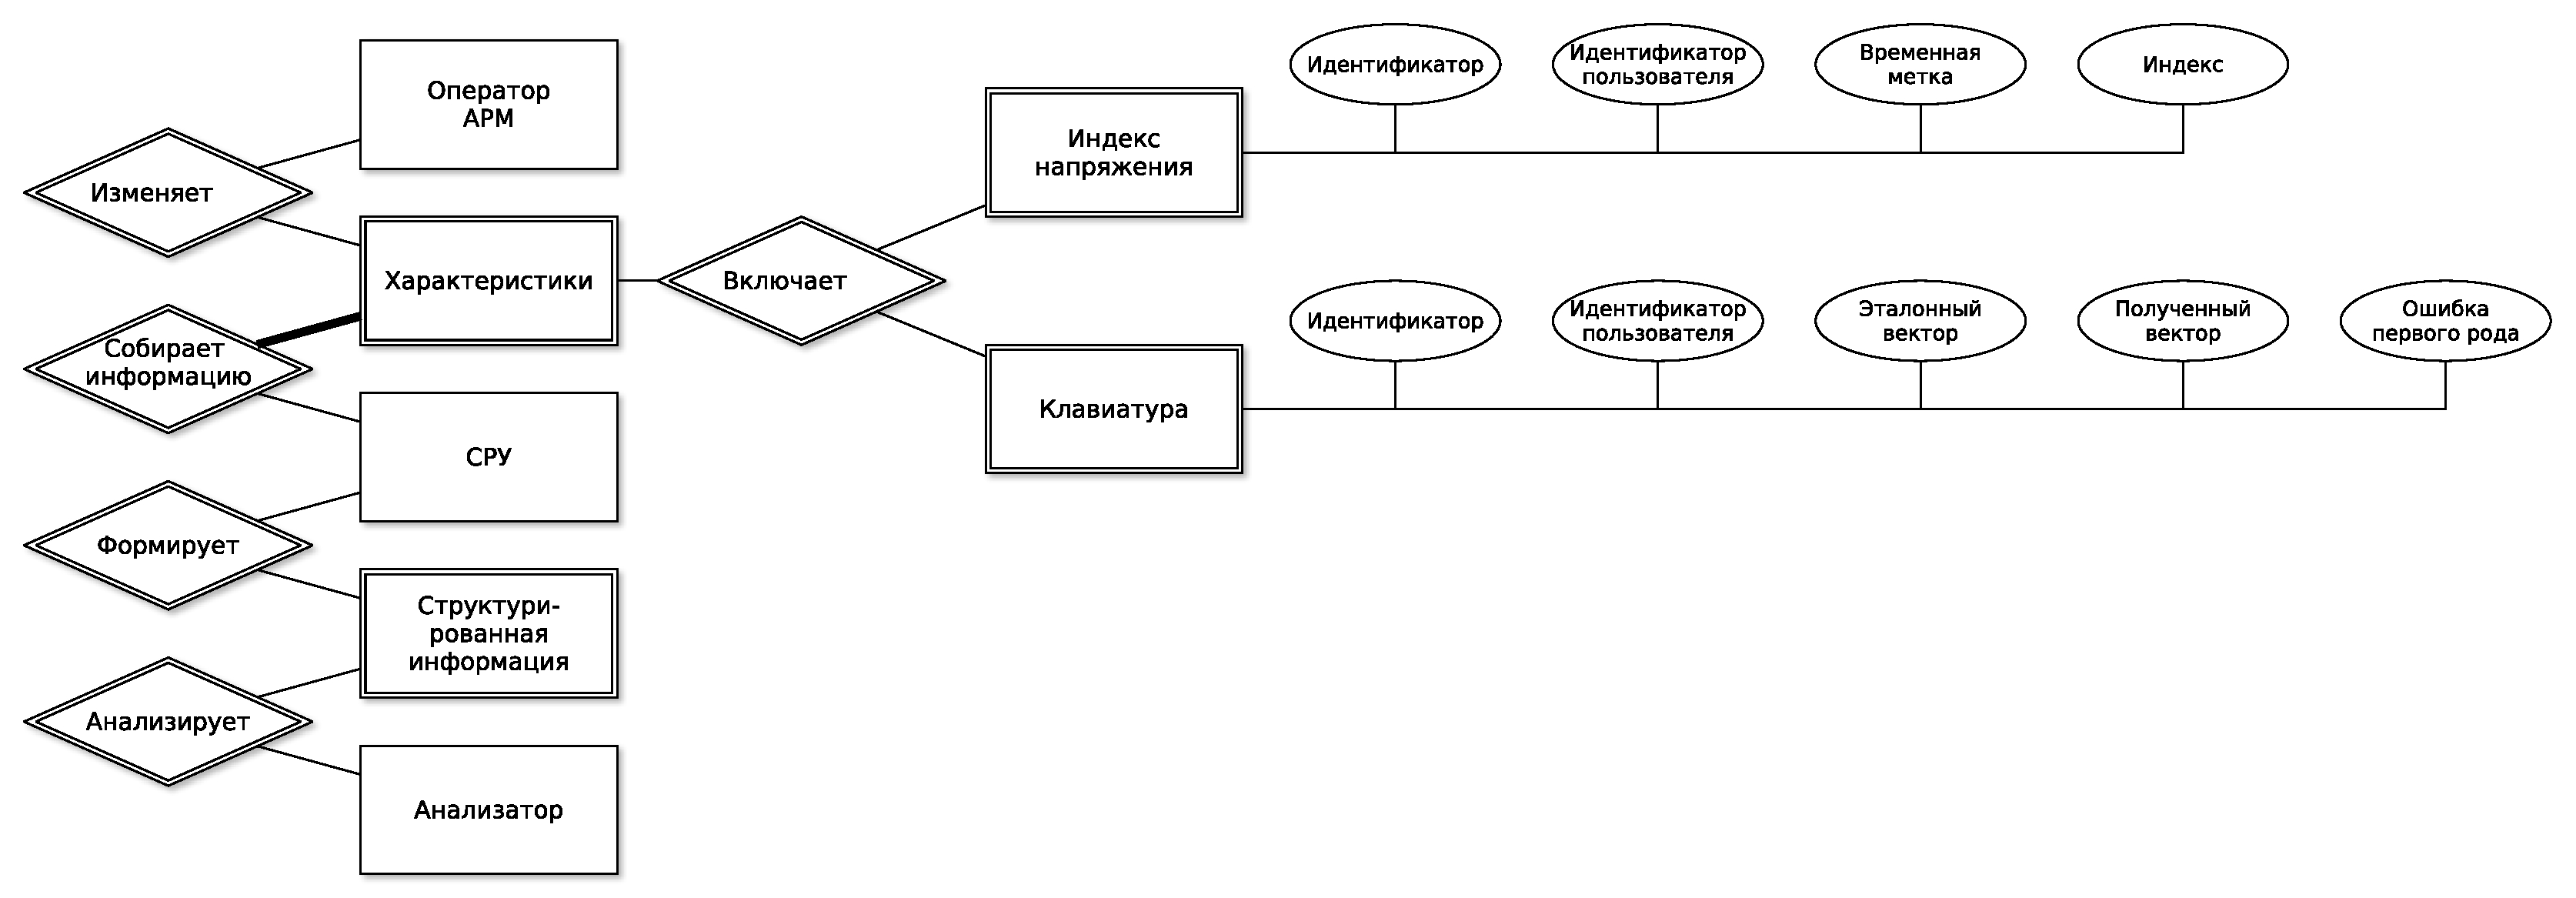
\includegraphics[width=\textwidth]{img/chenERDiagram.pdf}
	\caption{Диаграмма "сущность-связь"\ базы данных в нотации Чена.}
	\label{fig:chen}
\end{figure}

\subsection{IDEF0-диаграмма прикладной задачи}
На рисунках \ref{fig:idef:0}--\ref{fig:idef:1} предоставлена диаграмма IDEF0 прикладной задачи определения усталости оператора АРМ.

\begin{figure}[H]
	\centering
	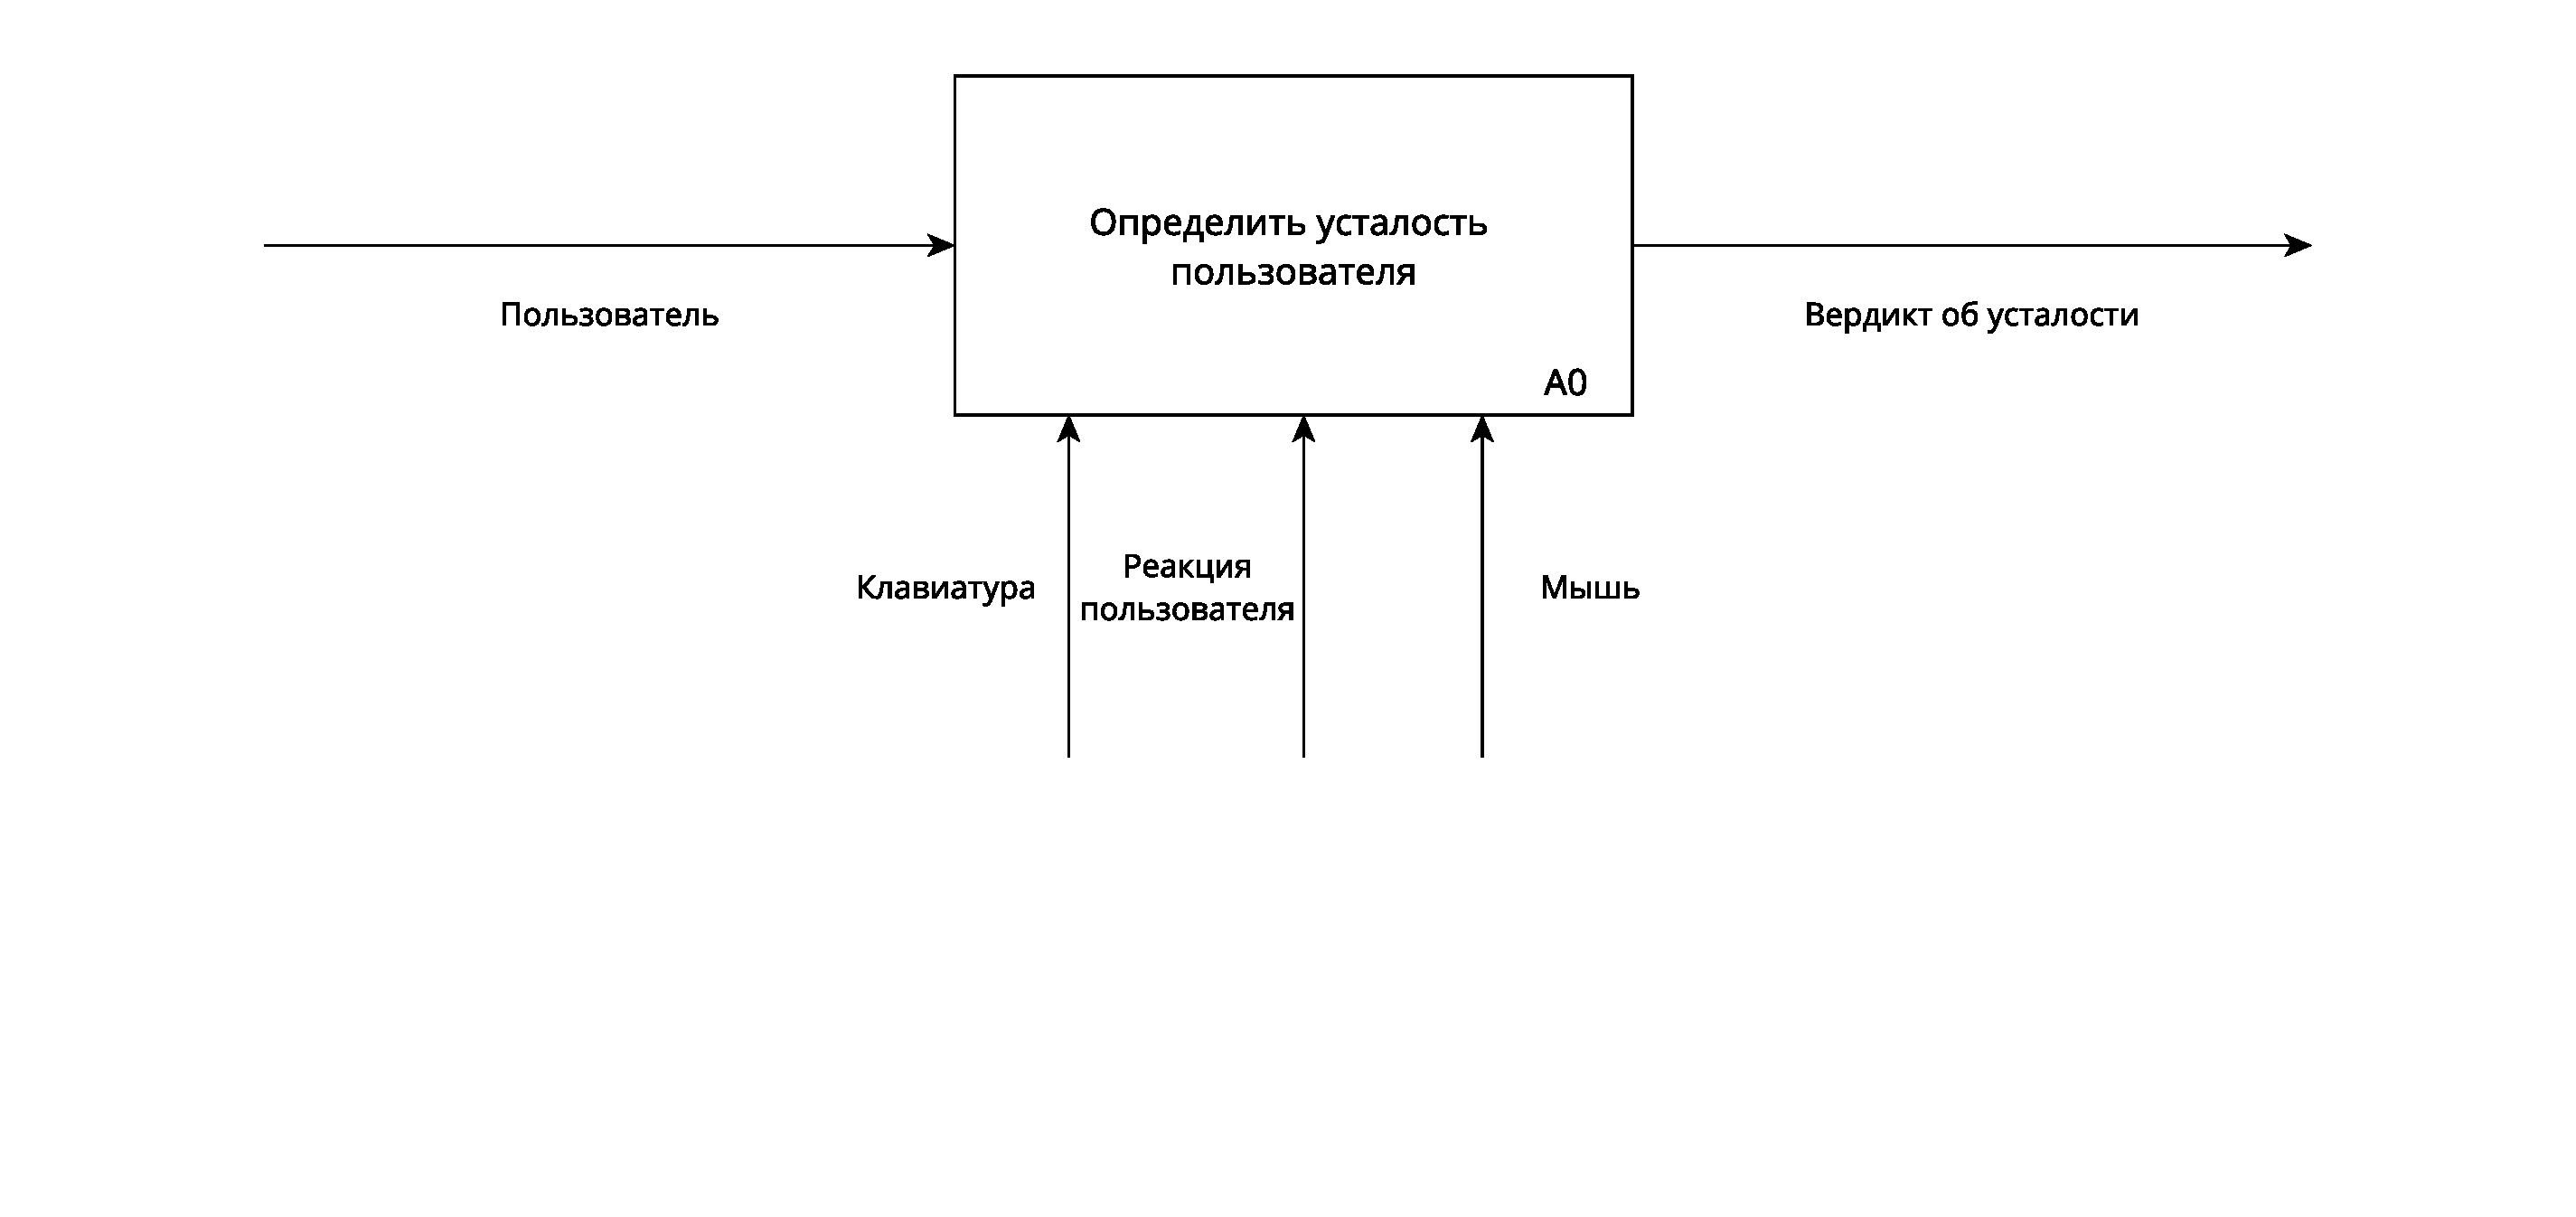
\includegraphics[width=\textwidth]{img/A0.pdf}
	\caption{IDEF0-диаграмма уровня A0.}
	\label{fig:idef:0}
\end{figure}

\begin{figure}[H]
	\centering
	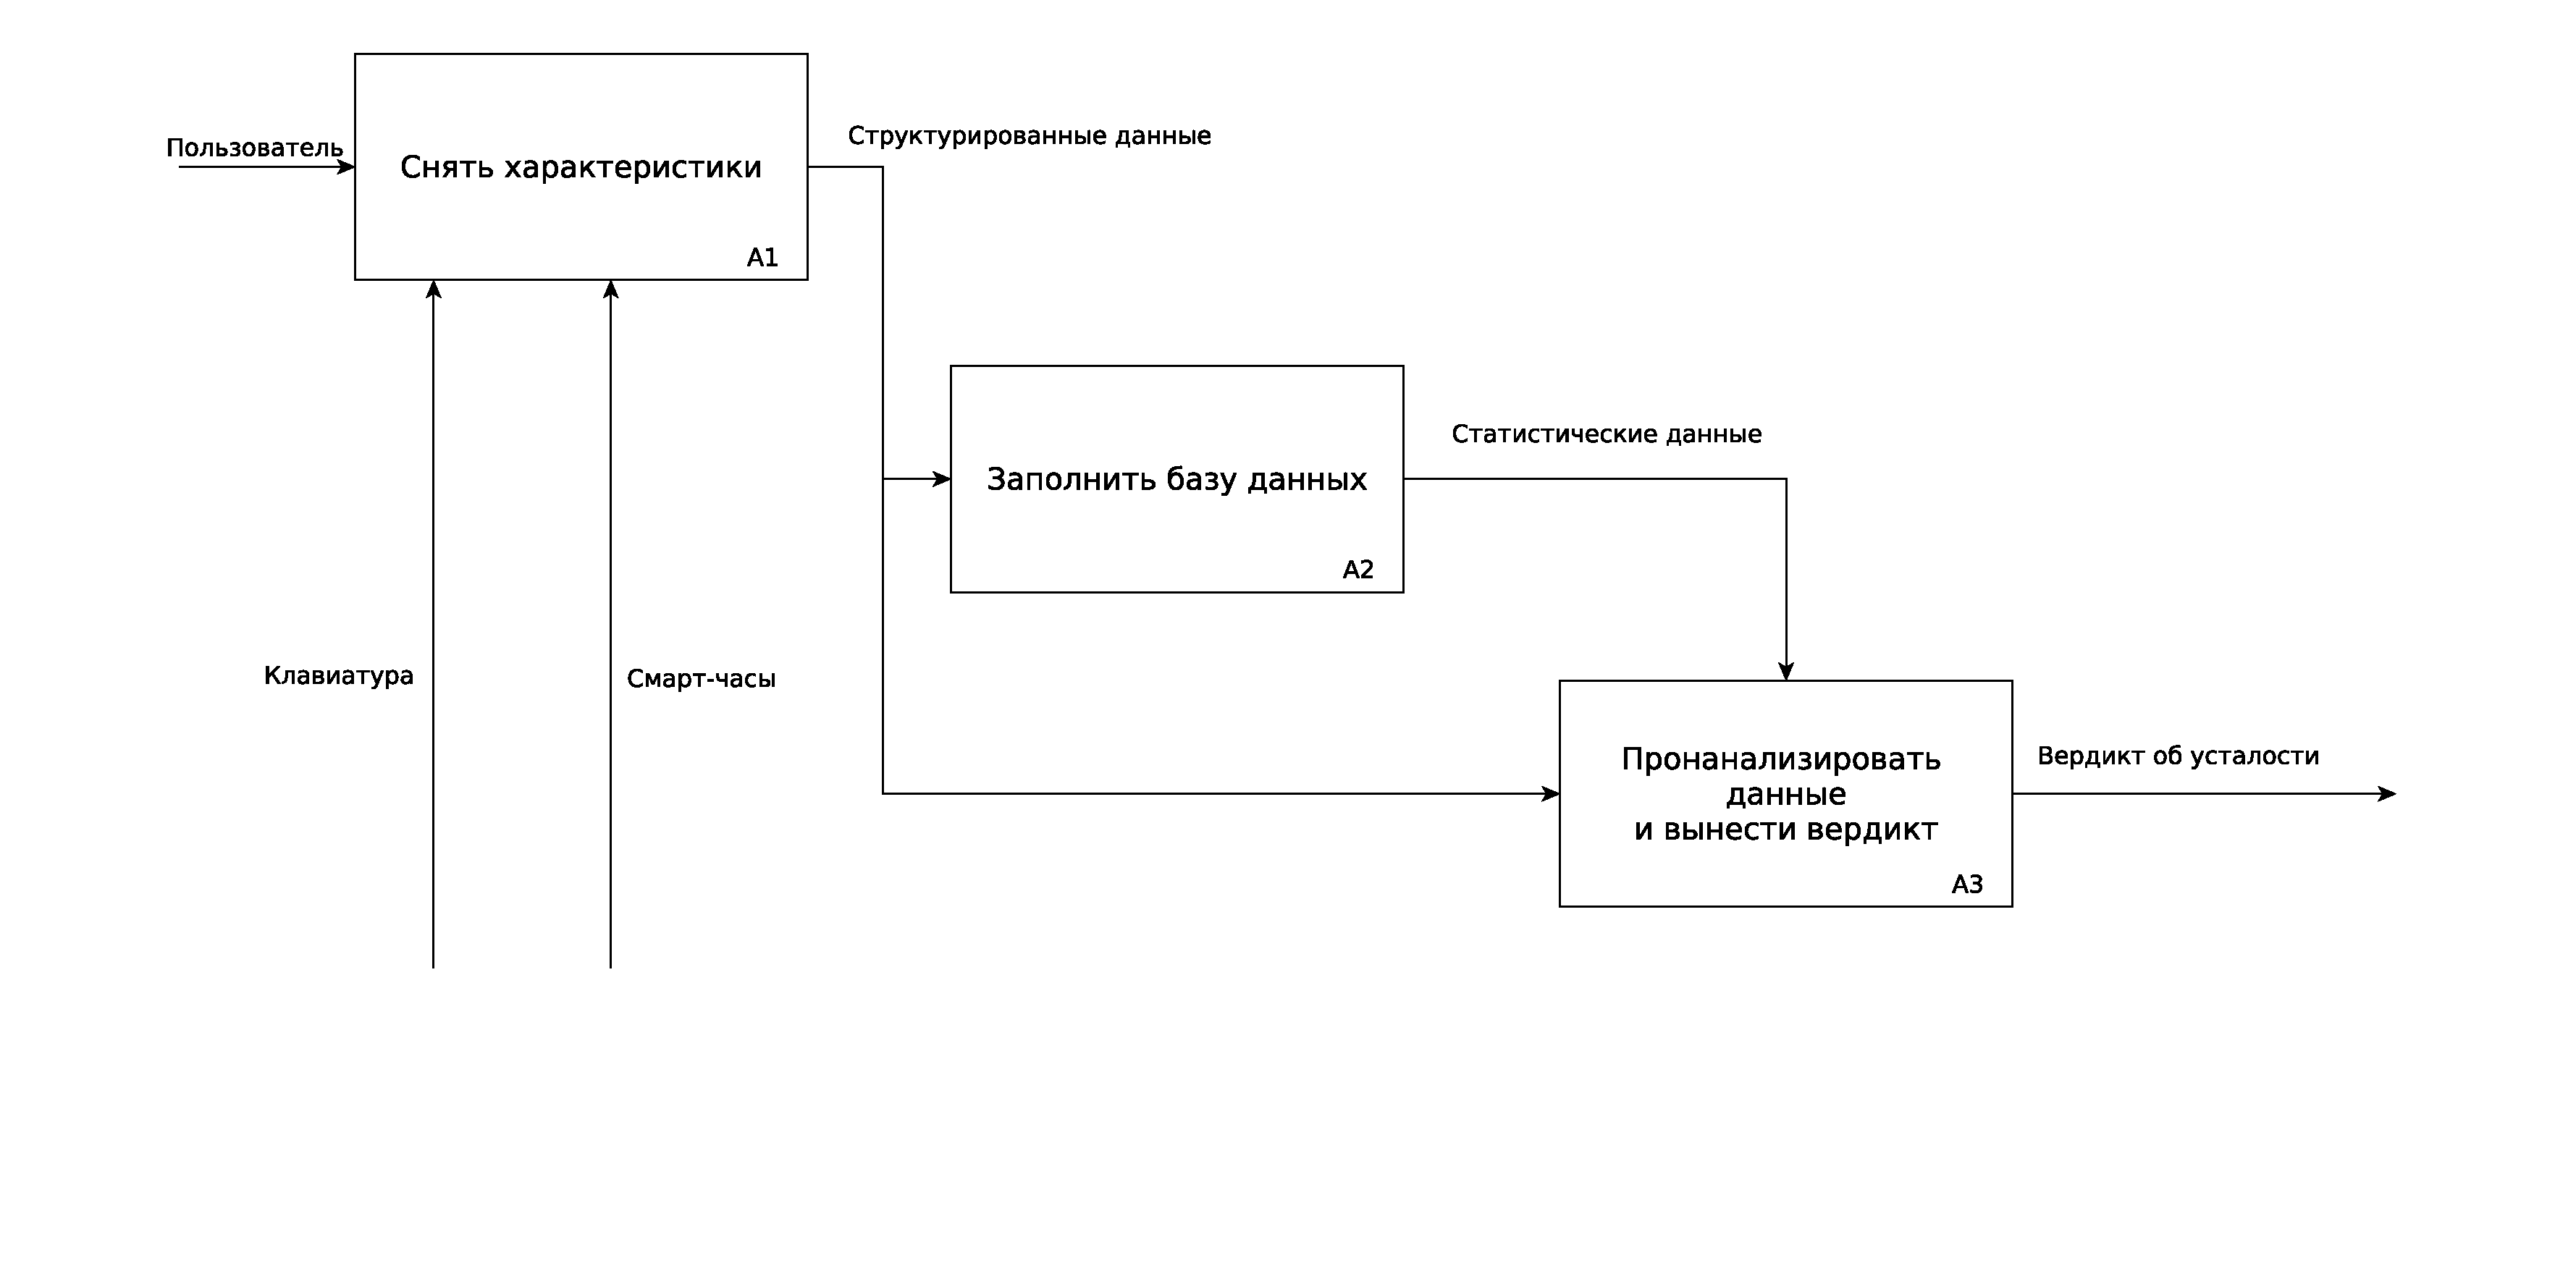
\includegraphics[scale=0.3]{img/A123.pdf}
	\caption{IDEF0-диаграмма уровня A1-A3.}
	\label{fig:idef:1}
\end{figure}

\subsection*{Вывод}
В разделе были представлены диаграмма вариантов использования, ER-диаграмма базы данных для хранения характеристик пользователя и IDEF0-диаграмма прикладной задачи.

Диаграмма вариантов использования позволила выделить 4 роли в системе: СРУ, анализатор характеристик, оператор АРМ, организм оператора АРМ.

Диаграмма "сущность-связь"\ включила в себя перечень выделенных характеристик из аналитического раздела и позволила описать базу данных для их хранения.

IDEF0-диаграмма позволила декомпозировать решаемую прикладную задачу.

\pagebreak